%Information relative au document
% !TEX encoding = MacOSRoman
\documentclass[a4paper,12pt]{report}

%Paquets
\usepackage[applemac]{inputenc}
\usepackage[T1]{fontenc}
\usepackage{lmodern,textcomp}
\usepackage[frenchb]{babel}
\usepackage{textcomp}
\usepackage{graphicx}
\usepackage{amsmath}


%D�but du rapport
\begin{document}

%Page de garde
\title{Rapport n�1 MT12}
\author{Alexandre Ballet et Simon LAURENT}
\date{Printemps 2016}
   
  %  \begin{minipage}{0.4\textwidth}
     % \begin{flushleft} \large
        %\emph{Enseignant :} M. Dajlil Kateb\\
        %\emph{Etablissement : } Universit� de Technologie de Compi�gne
      %\end{flushright}
    %\end{minipage}
\maketitle

%Table des mati�res
\tableofcontents

%Exercice 1
\chapter{S�rie de Fourier}
	\begin{enumerate}
		\item $f$ est $2\pi$ p�riodique, impaire et vaut $f(x)=1, x \in [0,\pi]$ \\ \\
		\begin{enumerate}
			\item Coefficients de Fourier \\ \\
			Les $a(i)$ �tant nuls. On obtient ainsi les coefficients suivants pour les $b(i)$ : \\ \\
			$b(1) = 1.273240$\\
			$b(2) = 0.000000$ \\
			$b(3) = 0.424413$\\
			$b(4) = 0.000000$\\
			$b(5) = 0.254648$\\
			$b(6) = -0.000000$\\
			$b(7) = 0.181891$\\
			$b(8) = 0.000000$\\
			$b(9) = 0.141471$\\
			$b(10) = 0.000000$\\
			\item S�rie de Fourier \\ \\

			\item Graphe original et ses dix premi�res approximations \\ \\
			\begin{figure}[h]
				\centering
				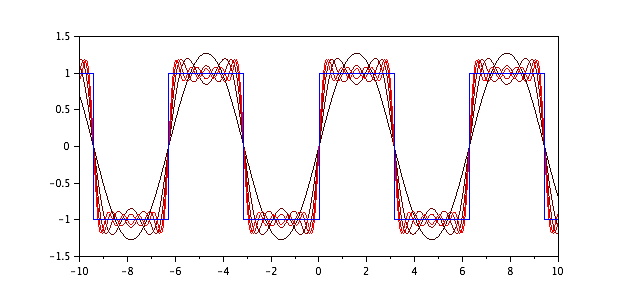
\includegraphics[scale=0.6]{ex1_fig1_1.png}\\*
				\caption{\label{ex1_figure1_1}Courbe de la fonction $f$.}
			\end{figure}\\
		
			\item Richesse fr�quentielle du signal \\ \\
			\begin{figure}[h]
				\centering
				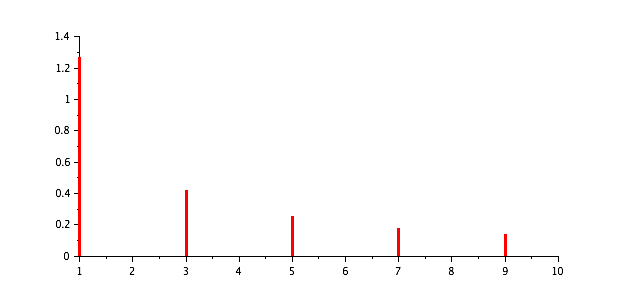
\includegraphics[scale=0.6]{ex1_fig1_2.png}\\*
				\caption{\label{ex1_figure1_2}Richesse du signal $f$.}
			\end{figure}\\
		\end{enumerate}
		\newpage
	
	%2.
		\item $f$ est $2\pi$ p�riodique, impaire et vaut $f(x)=x, x \in [0,\pi]$ \\ \\
		\begin{enumerate}
			\item Coefficients de Fourier \\ \\
			Les $a(i)$ �tant nuls. On obtient ainsi les coefficients suivants pour les $b(i)$ : \\ \\
			$b(1) = 2.000000\\
			b(2) = -1.000000\\
			b(3) = 0.666667\\
			b(4) 	= -0.500000\\
			b(5) = 0.400000\\
			b(6) = -0.333333\\
			b(7) = 0.285714\\
			b(8) = -0.250000\\
			b(9) = 0.222222\\
			b(10) = -0.200000$\\
			\item S�rie de Fourier \\ \\

			\item Graphe original et ses dix premi�res approximations \\ \\
			\begin{figure}[h]
				\centering
				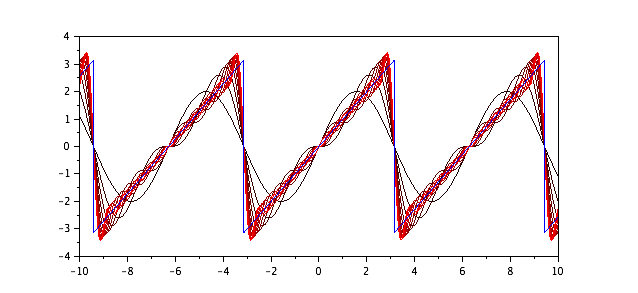
\includegraphics[scale=0.6]{ex1_fig2_1.png}\\*
				\caption{\label{ex1_figure2_1}Courbe de la fonction $f$.}
			\end{figure}\\
		
			\item Richesse fr�quentielle du signal \\ \\
			\begin{figure}[h]
				\centering
				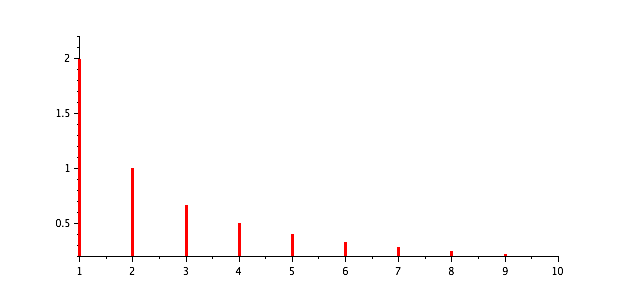
\includegraphics[scale=0.6]{ex1_fig2_2.png}\\*
				\caption{\label{ex1_figure2_2}Richesse du signal $f$.}
			\end{figure}\\
		\end{enumerate}
				\newpage
		
		%3.
		\item $f$ est $2\pi$ p�riodique, paire et vaut $f(x)=x, x \in [0,\pi]$ \\ \\
		\begin{enumerate}
			\item Coefficients de Fourier \\ \\
			Les $b(i)$ �tant nuls. On obtient ainsi les coefficients suivants pour les $a(i)$ : \\ \\
			$a(1) = 1.273240
a(2) = 0.000000\\
a(3) = 0.141471\\
a(4) = 0.000000\\
a(5) = 0.050930\\
a(6) = -0.000000\\
a(7) = 0.025984\\
a(8) = 0.000000\\
a(9) = 0.015719\\
a(10) = 0.000000$\\ \\
avec $a(0) = 3.141593$\\
			\item S�rie de Fourier \\ \\

			\item Graphe original et ses dix premi�res approximations \\ \\
			\begin{figure}[h]
				\centering
				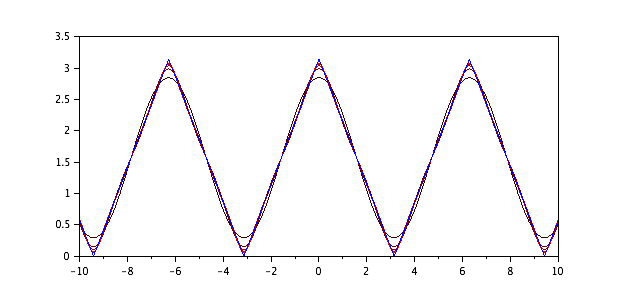
\includegraphics[scale=0.6]{ex1_fig3_1.png}\\*
				\caption{\label{ex1_figure3_1}Courbe de la fonction $f$.}
			\end{figure}\\
		
			\item Richesse fr�quentielle du signal \\ \\
			\begin{figure}[h]
				\centering
				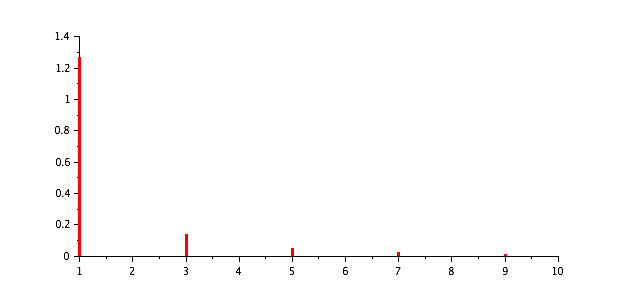
\includegraphics[scale=0.6]{ex1_fig3_2.png}\\*
				\caption{\label{ex1_figure3_2}Richesse du signal $f$.}
			\end{figure}\\
		\end{enumerate}
				\newpage
		
		%4.
		\item $f$ est $2\pi$ p�riodique, paire et vaut $f(x)=x^{2}, x \in [0,\pi]$ \\ \\
		\begin{enumerate}
			\item Coefficients de Fourier \\ \\
			Les $b(i)$ �tant nuls. On obtient ainsi les coefficients suivants pour les $a(i)$ : \\ \\
			$a(1) = -4.000000\\
a(2) = 1.000000\\
a(3) = -0.444444\\
a(4) = 0.250000\\
a(5) = -0.160000\\
a(6) = 0.111111\\
a(7) = -0.081633\\
a(8) = 0.062500\\
a(9) = -0.049383\\
a(10) = 0.040000$\\ \\
avec $a(0) = 6.579736$\\
			\item S�rie de Fourier \\ \\

			\item Graphe original et ses dix premi�res approximations \\ \\
			\begin{figure}[h]
				\centering
				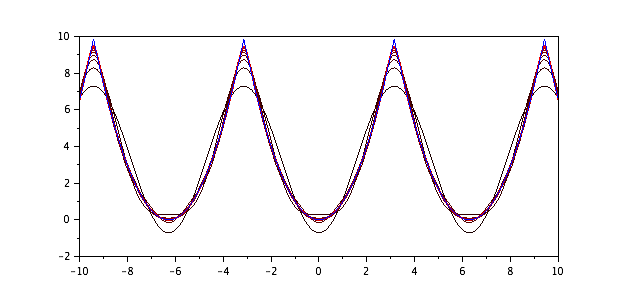
\includegraphics[scale=0.6]{ex1_fig4_1.png}\\*
				\caption{\label{ex1_figure4_1}Courbe de la fonction $f$.}
			\end{figure}\\
		
			\item Richesse fr�quentielle du signal \\ \\
			\begin{figure}[h]
				\centering
				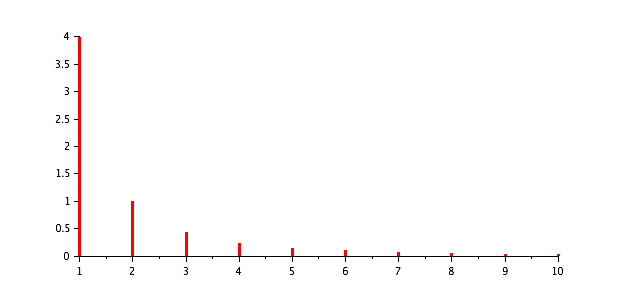
\includegraphics[scale=0.6]{ex1_fig4_2.png}\\*
				\caption{\label{ex1_figure4_2}Richesse du signal $f$.}
			\end{figure}\\
		\end{enumerate}
		\newpage
		
		%5.
		\item $f$ est $2\pi$ p�riodique, impaire et vaut $f(x)=x(\pi + |x|), x \in [-\pi,\pi]$ \\ \\
		\begin{enumerate}
			\item Coefficients de Fourier \\ \\
			Les $a(i)$ �tant nuls. On obtient ainsi les coefficients suivants pour les $b(i)$ : \\ \\
			$b(1) = 2.546479\\
b(2) = 0.000000\\
b(3) = 0.094314\\
b(4) = -0.000000\\
b(5) = 0.020372\\
b(6) = 0.000000\\
b(7) = 0.007424\\
b(8) = -0.000000\\
b(9) = 0.003493\\
b(10) = -0.000000\\$
			\item S�rie de Fourier \\ \\

			\item Graphe original et ses dix premi�res approximations \\ \\
			\begin{figure}[h]
				\centering
				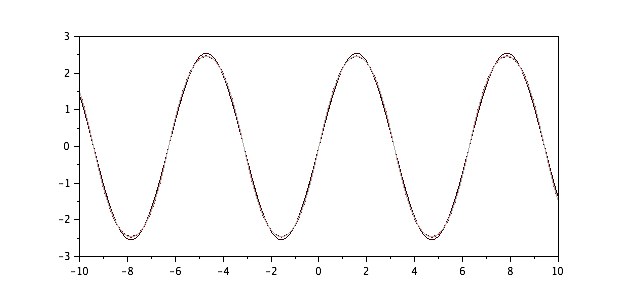
\includegraphics[scale=0.6]{ex1_fig5_1.png}\\*
				\caption{\label{ex1_figure5_1}Courbe de la fonction $f$.}
			\end{figure}\\
		
			\item Richesse fr�quentielle du signal \\ \\
			\begin{figure}[h]
				\centering
				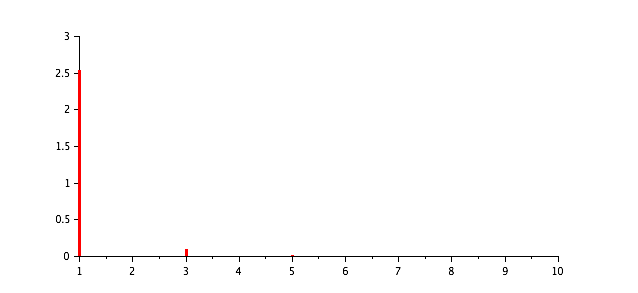
\includegraphics[scale=0.6]{ex1_fig5_2.png}\\*
				\caption{\label{ex1_figure5_2}Richesse du signal $f$.}
			\end{figure}\\
		\end{enumerate}

		
	\end{enumerate}
\newpage



	

%Exercice 2
\chapter{Classe de fonctions}
	\begin{enumerate}
	\item $f(x)=(sin\,x)^{1/3}$ \\ \\
	La fonction f est d�finie sur l'intervalle ($-\pi;\pi$). Elle est compos\'ee d'une fonction sinus, ce qui la rend impaire. Elle n'admet aucune valeur interdite et on a $f(0^+)=f(0^-)=\sqrt{0}=0$. Elle est donc continue.
	\begin{figure}[ht]
		\centering
		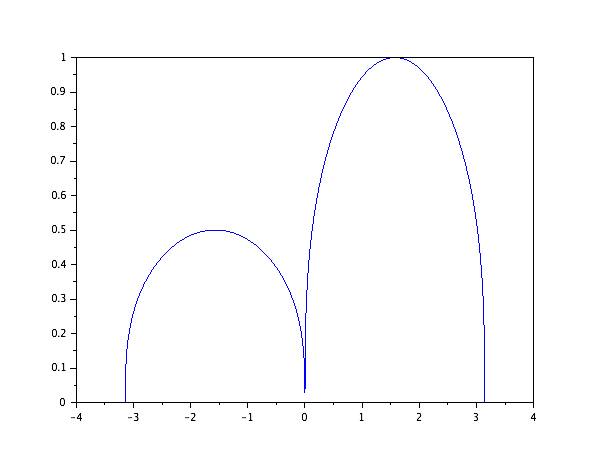
\includegraphics[scale=0.6]{ex2_fig1.png}
		\caption{\label{figure1}Courbe de la fonction $f$.}
		\end{figure}
		\\
	Sa d\'eriv\'ee est $f'(x)=\frac{1}{3} cos x (sin\,x)^{-2/3}$. Elle admet une asymptote verticale en $0$ et n'est donc pas continue.
	La fonction $f$ est continue mais non d\'erivable sur ($-\pi;\pi$).\\ \\
	% Faut-il ajouter le programme Scilab ? Que veux dire "Commenter" ?
	\item $f(x)=(sin\,x)^{4/3}$ \\ \\
	La fonction f est d�finie sur l'intervalle ($-\pi;\pi$). Elle n'admet aucune valeur interdite et on a $f(0^+)=f(0^-)=\sqrt[3]{0}=0$. Elle est donc continue.
	\begin{figure}[ht]
		\centering
		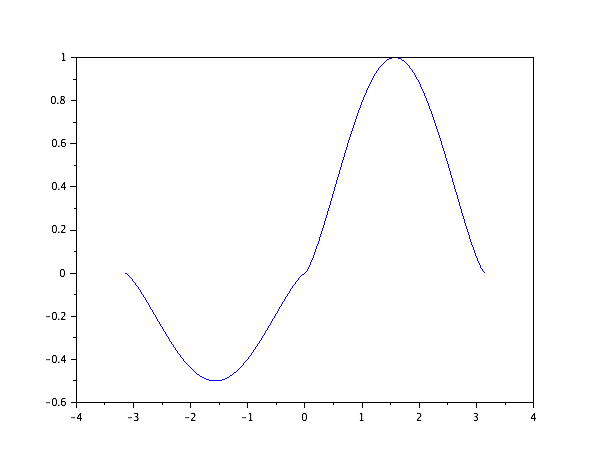
\includegraphics[scale=0.6]{ex2_fig2.png}
		\caption{\label{figure2}Courbe de la fonction $f$.}
		\end{figure}
		\\
	Sa d\'eriv\'ee est $f'(x)=\frac{4}{3} cos\,x (sin\,x)^{1/3}$. Elle n'admet pas d'asymptote et est donc continue.
	La fonction $f$ est continue et d\'erivable, donc r\'eguli\`ere.\\ \\
	\item $f(x)=
  \left\{
      \begin{aligned}
        cos\,x\quad , si\quad x > 0\\
        -cos\,x\quad ,si\quad x \le 0\\
      \end{aligned}
    \right.$ \\
	La fonction f est d�finie sur l'intervalle ($-\pi;\pi$). Elle n'admet aucune valeur interdite et on a $f(0^+)=1$ et $f(0^-)=-1$. Elle n'est donc pas continue en 0.
	\begin{figure}[ht]
		\centering
		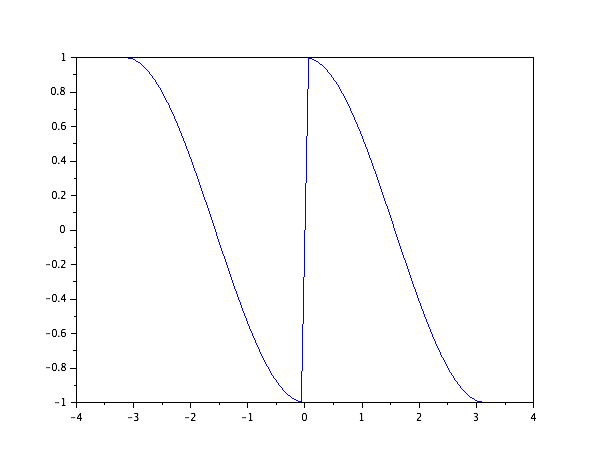
\includegraphics[scale=0.6]{ex2_fig3.png}
		\caption{\label{figure3}Courbe de la fonction $f$.}
		\end{figure}
		\\
	Elle est d\'erivable par morceaux et sa d\'eriv\'ee est $f'(x)=
  \left\{
      \begin{aligned}
        -sin\,x\quad , si\quad x > 0\\
        sin\,x\quad ,si\quad x \le 0\\
      \end{aligned}
    \right.$ \\
	La fonction $f$ est continue par morceaux et d\'erivable par morceaux, donc r\'eguli\`ere par morceaux.\\ \\
	\item $f(x)=
  \left\{
      \begin{aligned}
        sin\,x\quad , si\quad x > 0\\
        -sin\,2x\quad ,si\quad x \le 0\\
      \end{aligned}
    \right.$ \\ \\
	La fonction f est d�finie sur l'intervalle ($-\pi;\pi$). Elle n'admet aucune valeur interdite et on a $f(0^+)=f(0^-)=0$. Elle est donc continue.
	\begin{figure}[ht]
		\centering
		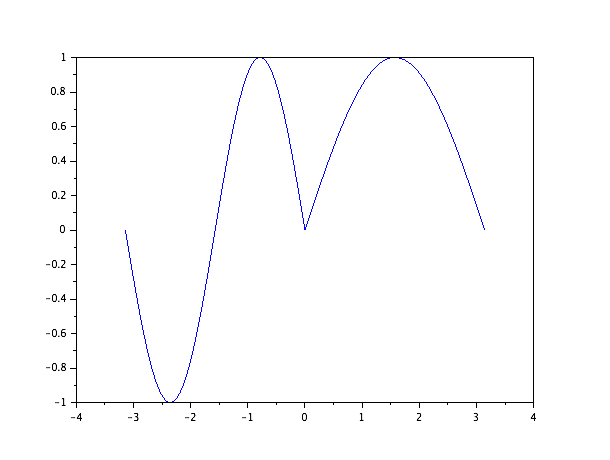
\includegraphics[scale=0.6]{ex2_fig4.png}
		\caption{\label{figure4}Courbe de la fonction $f$.}
		\end{figure}
		\\
	Elle est d\'erivable par morceaux et sa d\'eriv\'ee est $f'(x)=
  \left\{
      \begin{aligned}
        cos\,x\quad , si\quad x > 0\\
        -2cos\,2x\quad ,si\quad x \le 0\\
      \end{aligned}
    \right.$ \\
	La fonction $f$ est continue et d\'erivable par morceaux, donc r\'eguli\`ere par morceaux.\\ \\
	\item $f(x)=
  \left\{
      \begin{aligned}
        (sin\,x)^{1/5}\quad , si\quad x < \pi/2\\
        -cos\,x\quad ,si\quad x \ge \pi/2\\
      \end{aligned}
    \right.$ \\ \\
	La fonction f est d�finie sur l'intervalle ($-\pi;\pi$). Elle n'admet aucune valeur interdite et on a $f(0^+)=f(0^-)=\sqrt{0}=0$ et $f(\pi/2)=0$ et $\lim\limits_{\substack{x \rightarrow \pi/2 \\ x>\pi/2}} f(x)$. Elle est continue en 0 mais pas en $\pi/2$, elle est donc continue par morceaux.
	\begin{figure}[ht]
		\centering
		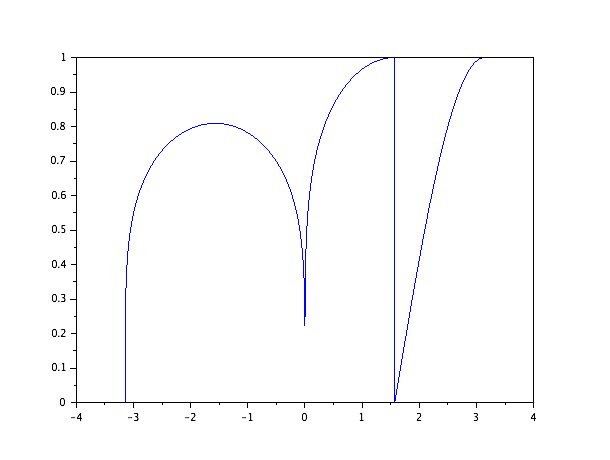
\includegraphics[scale=0.6]{ex2_fig5.png}
		\caption{\label{figure5}Courbe de la fonction $f$.}
		\end{figure}
		\\
	Elle est d\'erivable par morceaux et sa d\'eriv\'ee est $f'(x)=
  \left\{
      \begin{aligned}
        \frac{1}{5}cos\,x\,(sin\,x)^{1/5}\quad , si\quad x < \pi/2\\
        sin\,x\quad ,si\quad x \ge \pi/2\\
      \end{aligned}
    \right.$ \\
	La fonction $f$ est continue par morceaux et d\'erivable par morceaux, donc r\'eguli\`ere par morceaux.\\ \\
	\end{enumerate}
%Exercice 3
\chapter{Ph�nom�ne de Gibbs}
\section{D\'emonstration}
Soit f la fonction 2$\pi$-p\'eriodique et impaire telle que $f(x) = 1$ sur $[0; \pi]$.\\

Nous allons montrer que $S_{f(x)}=\frac{4}{\pi}\sum\limits_{n=0}^{\infty}\frac{sin(2k-1)}{2k-1}$\\\\

Nous savons que $S_{f(x)}=\sum\limits_{n=0}^{\infty} b_{n}sin(nx)$, car f est impaire.\\
Or, \begin{large}
$b_{n}=\frac{1}{\pi}\int_{-\pi}^{\pi}f(x)sin(nx)$\\
		 $=\frac{1}{\pi}\int_{-\pi}^{0}f(x)sin(nx)\,+\,\frac{1}{\pi}\int_{0}^{\pi}f(x)sin(nx)$\\
		 $=-\frac{1}{\pi}\int_{-\pi}^{0}sin(nx)\,+\,\frac{1}{\pi}\int_{0}^{\pi}sin(nx)$\\
		 $=\frac{1}{\pi}\int_{0}^{\pi}sin(nx)\,+\,\frac{1}{\pi}\int_{0}^{\pi}sin(nx)$\\
		 $=\frac{2}{\pi}\int_{0}^{\pi}sin(nx)$\\
		 $=\frac{2}{\pi}\lbrack\frac{-cosnx}{k}\rbrack_0^\pi$\\
		 $=\frac{2}{\pi}(-\frac{cosn\pi}{n}+\frac{1}{n})$\\
		 $=\frac{2}{\pi}(-\frac{cosn\pi}{n}+\frac{1}{n})$\\
	\end{large}
D'o� \begin{large}
$S_{f(x)}=\frac{1}{\pi}\int_{-\pi}^{\pi}f(x)sin(nx)$\\
		$=\frac{2}{\pi}\sum\limits_{n=0}^{\infty}\frac{1-cosnx}{n}sinnx$\\
		$=\frac{2}{\pi}\sum\limits_{n=0}^{\infty}\frac{1-(-1)^{n}}{n}sinnx$\\
		$=\frac{2}{\pi}\sum\limits_{n\,pair}^{\infty}\frac{1-(-1)^{n}}{n}sinnx\,+\,\frac{2}{\pi}\sum\limits_{n\,impair}^{\infty}\frac{1-(-1)^{n}}{n}sinnx$\\
		$=\frac{4}{\pi}\sum\limits_{n\,impair}^{\infty}\frac{sinnx}{n}$\\
		$=\frac{4}{\pi}\sum\limits_{n=1}^{\infty}\frac{sin(2k-1)x}{2k-1}$, o� $n=2k-1$\\
	\end{large}


%Exercice 4
\chapter{Application des s�rie de Fourier}
\section{La corde pinc�}
\section{La corde frapp�e}

%Exercice 5
\chapter{Equation de la chaleur}

%Compl�ment au TP
\chapter{Compl�ments}
\section{Finance}
\section{Informatique}

%Test de texte
Comme le disait Jean de la Fontaine dans sa fable :
\begin{quote}
Rien de sert de courir, il faut partir � point.
\end{quote}


\end{document}